\begin{figure*}[t]
    \centering
    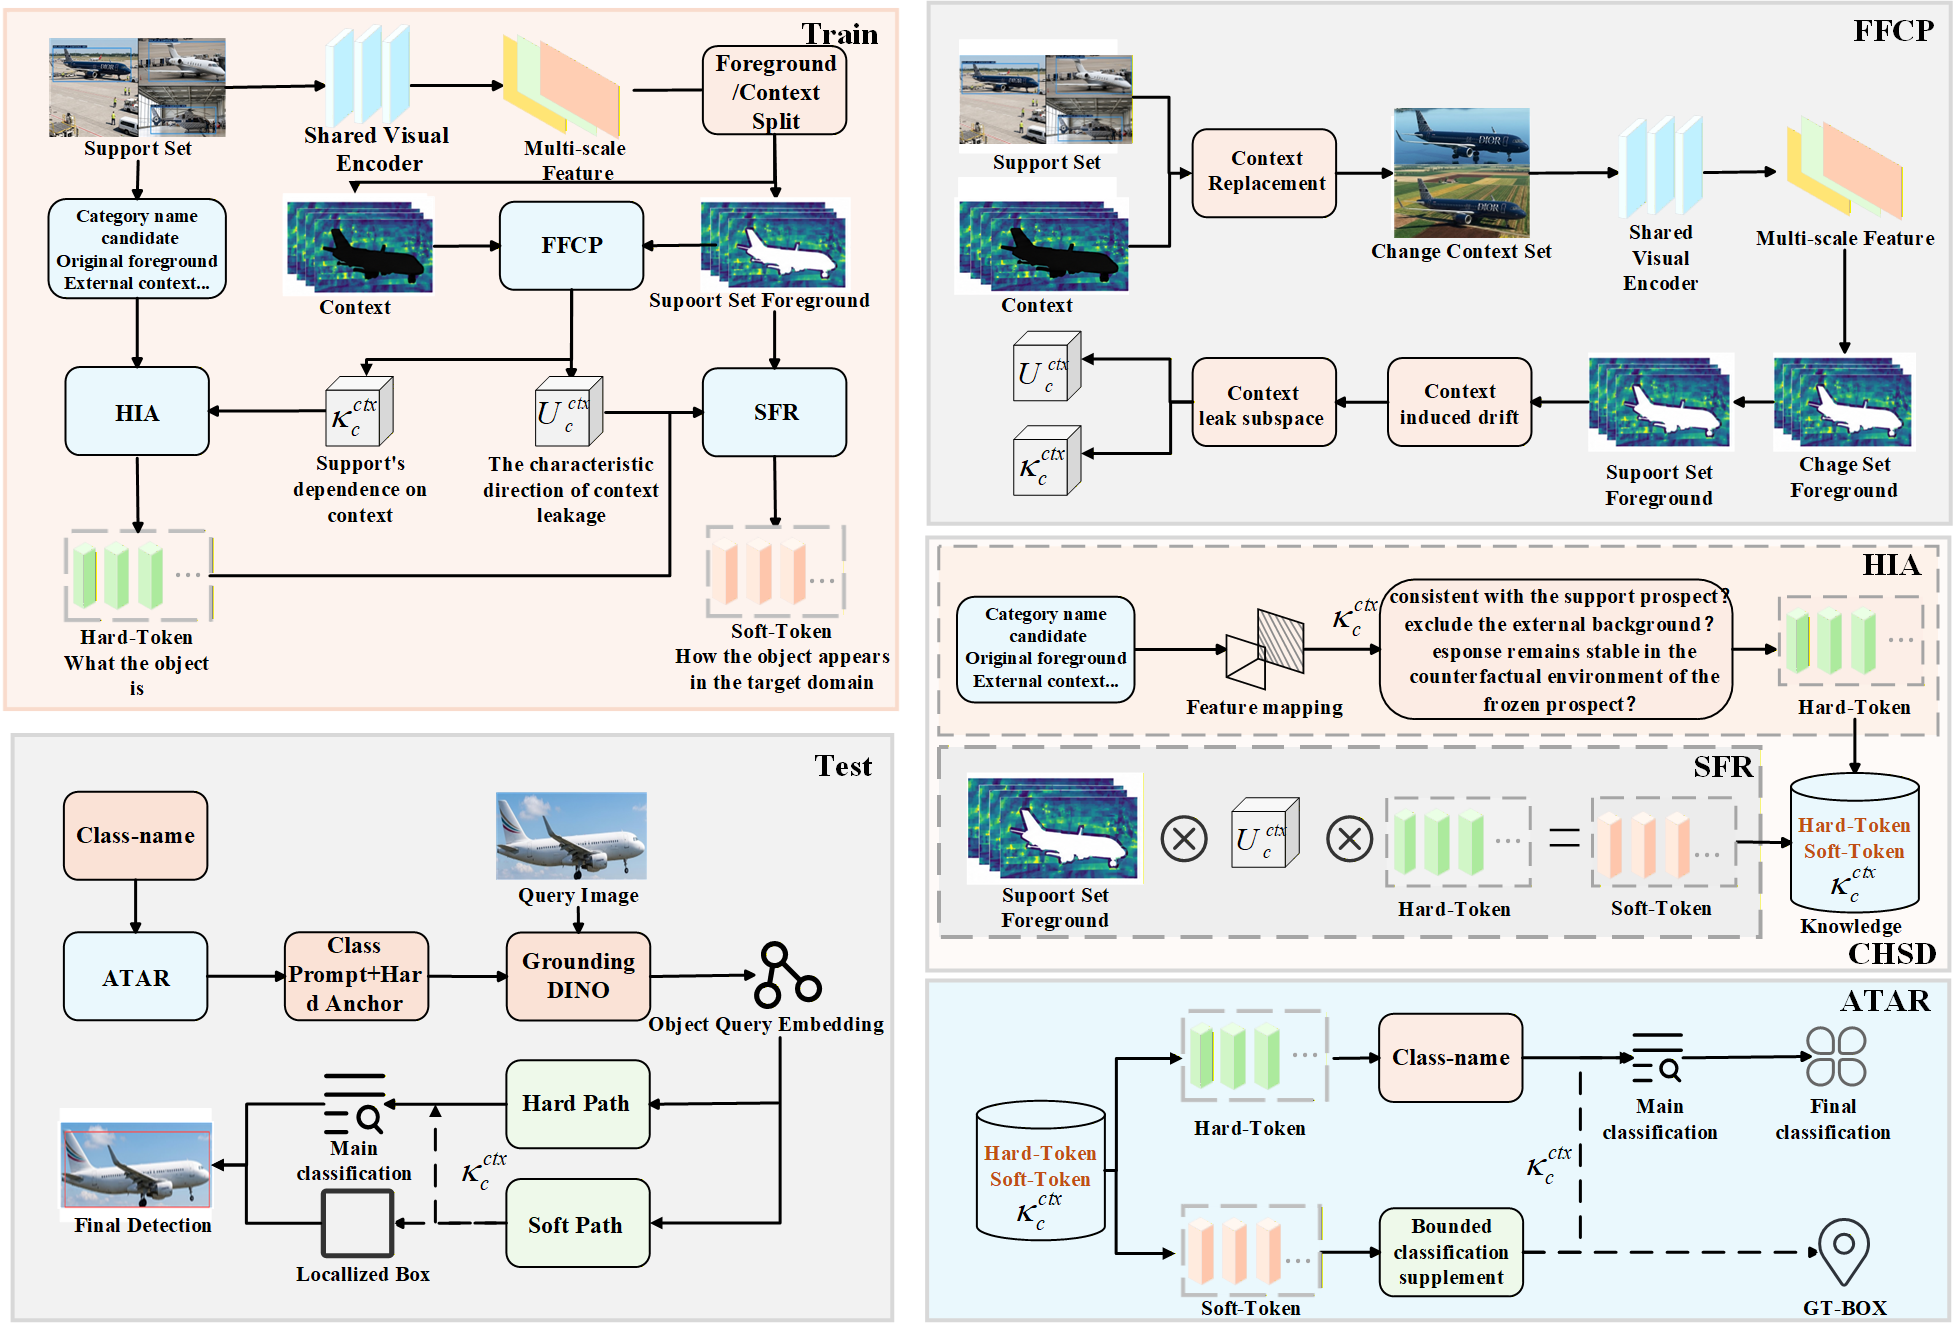
\includegraphics[width=\textwidth]{fig/method_overview.png}
    \caption{\textbf{Knowledge-enhanced Hard--Soft framework.} (1) Foreground-Frozen Context Probing (FFCP) modifies only the support context and estimates a class-wise context-sensitive subspace. (2) Context-Constrained Hard--Soft Decomposition (CHSD) builds a bounded Hard identity anchor and a context-cleaned Soft appearance residual. (3) Grounding DINO first produces its ordinary query predictions. (4) Asymmetric Task-Authority Routing (ATAR) uses Hard--Soft agreement and baseline-query uncertainty to authorize a bounded cosine class correction while leaving the localization output unchanged.}
    \label{fig:overview}
\end{figure*}


\section{Method}
\label{sec:method}

Figure~\ref{fig:overview} presents our knowledge-enhanced Hard-Soft framework. We formulate target-domain adaptation as a constrained knowledge update rather than a complete prototype transfer. Foreground-Frozen Context Probing (FFCP) measures how support context perturbs an otherwise unchanged foreground representation. Context-Constrained Hard-Soft Decomposition (CHSD) then constructs a Hard identity anchor and a reliability-weighted, context-cleaned Soft prototype. Finally, Asymmetric Task-Authority Routing (ATAR) uses Hard--Soft agreement and baseline-query uncertainty to bound a cosine class correction in a single Grounding DINO detector~\cite{groundingdino}. Hard knowledge controls whether the Soft direction is trustworthy; it is not injected as an independent classifier, and the baseline localization path remains unchanged. We refer to the complete instantiation as S2H-CD-FSOD.

\subsection{Preliminaries}
\label{sec:preliminaries}

Let $\mathcal C$ denote the target-category set. Following standard CD-FSOD protocols~\cite{cdvito,yu2026}, the support set of category $c$ and the predictions for an unlabeled query image $x_q$ are
\begin{equation}
\begin{aligned}
\mathcal S_c^K
&=\{(x_{c,i},b_{c,i},c)\}_{i=1}^{K},
\quad K\in\{1,5,10\},\\
\widehat{\mathcal Y}_q
&=\{(\hat b_j,\hat y_j,\hat p_j)\}_{j=1}^{M'}.
\end{aligned}
\label{eq:problem}
\end{equation}
where $x_{c,i}$ and $b_{c,i}$ denote a support image and its annotated bounding box, respectively. At inference time, neither query boxes nor query labels are available. Category names are obtained from the support annotations and used to form the textual prompt, but support knowledge never directly assigns a label to a query object.

Grounding DINO aligns image regions with textual phrases and performs language-guided query selection before Transformer decoding~\cite{groundingdino}. We keep this open-vocabulary path unchanged and apply support calibration only after the ordinary decoder logits are available. For each category, our support-side procedure constructs
\begin{equation}
\mathcal K_c=(\mathbf h_c,\mathbf s_c,
\kappa_c^{\mathrm{ctx}}),
\label{eq:knowledge_cache}
\end{equation}
where $\mathbf h_c$ is the Hard identity anchor, $\mathbf s_c$ denotes Soft foreground-appearance knowledge, and $\kappa_c^{\mathrm{ctx}}\in[0,1)$ measures the dependence of the support representation on external context.

\subsection{Foreground-Frozen Context Probing}
\label{sec:ffcp}

Although support features are pooled from annotated boxes, the visual encoder can still transmit information from runways, water, roads, or industrial substrates. FFCP estimates this influence through foreground-preserving interventions. We dilate each support box to obtain a protection mask $M_{c,i}$ that covers the target and its boundary. The $r$-th intervened support image is
\begin{equation}
\tilde x_{c,i}^{(r)}
=M_{c,i}\odot x_{c,i}
+(1-M_{c,i})\odot B_i^{(r)},
\label{eq:counterfactual}
\end{equation}
where $B_i^{(r)}$ is obtained through in-domain background exchange, category-mismatched exchange, or context neutralization. The protected pixels, box geometry, viewpoint, scale, resolution, and foreground texture remain unchanged. These intervened views serve only as probes and are never counted as additional shots.

The original image, its intervened counterpart, and a reconstruction control are processed by the same frozen visual encoder. RoIAlign and attention pooling extract the target representations $\mathbf f_{c,i}$, $\tilde{\mathbf f}_{c,i}^{(r)}$, and $\mathbf f_{c,i}^{\mathrm{rec}}$ from the same box. The reconstruction control uses the same synthesis pipeline but reinserts the original context. We define the resulting context-induced drift as
\begin{equation}
\mathbf d_{c,i}^{(r)}
=\big(\mathbf f_{c,i}-\tilde{\mathbf f}_{c,i}^{(r)}\big)
-\big(\mathbf f_{c,i}-\mathbf f_{c,i}^{\mathrm{rec}}\big),
\label{eq:context_drift}
\end{equation}
The second term removes drift caused by compositing and resampling. A nonzero residual indicates that external context perturbs the protected target representation.

Let $\mathbf D_c$ stack all drift vectors for category $c$. We retain its leading right-singular vectors and quantify the normalized leakage energy as
\begin{equation}
\begin{aligned}
\mathbf U_c^{\mathrm{ctx}}
&=\operatorname{TopSVD}(\mathbf D_c,r),\\
e_c^{\mathrm{ctx}}
&=\frac{1}{KR}\sum_{i,r}
\frac{\|({\mathbf U_c^{\mathrm{ctx}}})^\top
\mathbf d_{c,i}^{(r)}\|_2^2}
{\|\mathbf f_{c,i}\|_2^2+\epsilon},\\
\kappa_c^{\mathrm{ctx}}
&=1-\exp(-e_c^{\mathrm{ctx}}).
\end{aligned}
\label{eq:context_subspace}
\end{equation}
The columns of $\mathbf U_c^{\mathrm{ctx}}$ describe \emph{where} context enters the target representation, while $\kappa_c^{\mathrm{ctx}}$ quantifies \emph{how strongly} the support depends on context. For 1-shot adaptation, we restrict the rank and shrink the class-specific estimate toward a cross-category drift subspace. As $K$ increases, the class-specific estimate receives greater weight.

\subsection{Context-Constrained Hard-Soft Decomposition}
\label{sec:chsd}

FFCP identifies context-sensitive directions but does not determine category identity. CHSD therefore decomposes support knowledge in two stages: it first identifies invariant category factors and then extracts adaptable target-domain appearance.

For category $c$, we obtain a compact candidate set from its name, synonyms, and deterministic structural attributes. For example, valid identity hypotheses for an airplane include wings, a fuselage, and a tail, but exclude a top-down view, low resolution, or a runway. These candidates are drawn from predefined structural templates rather than free-form target-domain generation. Recent CD-FSOD methods have demonstrated that support prototypes can complement pretrained textual semantics~\cite{lmp,astigmatism}; CHSD additionally determines whether each candidate is sufficiently reliable to alter category knowledge. After mapping the textual and visual features into the normalized Grounding DINO alignment space, we measure counterfactual instability and define the qualification score for attribute $\mathbf a_{c,l}$ as
\begin{equation}
\begin{aligned}
\Delta_{c,l}^{\mathrm{cf}}
&=\frac{1}{KR}\sum_{i,r}
\left|
\operatorname{sim}(\mathbf a_{c,l},\mathbf f_{c,i})
-\operatorname{sim}(\mathbf a_{c,l},
\tilde{\mathbf f}_{c,i}^{(r)})
\right|,\\
q_{c,l}={}&
\operatorname{sim}(\mathbf a_{c,l},\bar{\mathbf f}_c^{\mathrm{fg}})
-\lambda_b
\big[\operatorname{sim}(\mathbf a_{c,l},
\bar{\mathbf f}_c^{\mathrm{ctx}})\big]_+\\
&-\lambda_{\mathrm{cf}}\Delta_{c,l}^{\mathrm{cf}}
-\lambda_\kappa\kappa_c^{\mathrm{ctx}}.
\end{aligned}
\label{eq:hard_qualification}
\end{equation}
The four terms enforce foreground support, reject positive context correlation, penalize intervention-sensitive attributes, and reduce the qualification scores of categories whose support is globally context dependent, respectively. Thus, $\kappa_c^{\mathrm{ctx}}$ influences Hard construction rather than being used only at query time.

Only candidates whose scores exceed the threshold $\xi_H$ are retained. Their weighted aggregate is projected onto an $\ell_2$ ball before being added to the base category embedding $\mathbf t_c^0$:
\begin{equation}
\begin{aligned}
\mathcal V_c&=\{l\mid q_{c,l}\geq\xi_H\},\qquad
w_{c,l}=\operatorname{softmax}_{l\in\mathcal V_c}
(q_{c,l}/T_q),\\
\Delta\mathbf h_c
&=\Pi_{\|\cdot\|_2\leq\rho_H}
\left(\sum_{l\in\mathcal V_c}w_{c,l}\mathbf a_{c,l}\right),\\
\mathbf h_c&=\operatorname{Norm}
(\mathbf t_c^0+\Delta\mathbf h_c).
\end{aligned}
\label{eq:hard_anchor}
\end{equation}
If no attribute qualifies, we set $\Delta\mathbf h_c=\mathbf 0$ and recover the original category representation. The radius $\rho_H$ prevents a few support instances from arbitrarily rewriting pretrained category semantics.

Hard knowledge should not absorb target-domain appearance factors such as nadir viewpoints, compressed scale, blur, or low-resolution texture. We map the base identity and accepted attributes into the visual space and orthonormalize them to obtain the identity subspace $\mathbf U_c^H$. We remove context leakage only within the identity complement, thereby preventing context suppression from erasing category-defining directions. The Soft residual for support instance $i$ is
\begin{equation}
\begin{aligned}
\mathbf P_c^H&=\mathbf U_c^H({\mathbf U_c^H})^\top,\\
\bar{\mathbf U}_c^{\mathrm{ctx}}
&=\operatorname{Orth}\!\left[
(\mathbf I-\mathbf P_c^H)\mathbf U_c^{\mathrm{ctx}}
\right],\\
\mathbf r_{c,i}^{\mathrm{app}}
&=(\mathbf I-\mathbf P_c^H)
\left(\mathbf I-\bar{\mathbf U}_c^{\mathrm{ctx}}
({\bar{\mathbf U}_c^{\mathrm{ctx}}})^\top\right)
\mathbf f_{c,i}.
\end{aligned}
\label{eq:soft_residual}
\end{equation}
Counterfactual background features never enter Soft knowledge. FFCP identifies the directions to be removed, whereas the retained appearance is always derived from the original support foreground.

We robustly aggregate the residuals and apply shot-aware shrinkage:
\begin{equation}
\mathbf s_c=(1-\alpha_K)
\operatorname{RobustMean}
\big(\{\mathbf r_{c,i}^{\mathrm{app}}\}_{i=1}^{K}\big),
\qquad
\alpha_K=\frac{\xi}{K+\xi}.
\label{eq:soft_aggregation}
\end{equation}
This estimator remains conservative in the 1-shot setting and places progressively greater trust in the target-domain residual as more support instances become available. It changes only the stability of knowledge estimation; the network architecture remains identical across the 1-, 5-, and 10-shot protocols.

\subsection{Asymmetric Task-Authority Routing}
\label{sec:atar}

ATAR connects the support-side decomposition to query detection without
granting a noisy few-shot prototype unrestricted authority. Grounding DINO
first produces decoded query embeddings $\mathbf z_j$, boxes $\mathbf b_j$,
and category logits $L^0_{j,c}$ from the ordinary textual prompts. The Hard
anchor is used as a reliability signal rather than being injected into the
text or added directly to the logits. This preserves the pretrained
vision--language boundary and lets support knowledge act only through a
bounded calibration interface.

For category $c$, CHSD supplies a prototype reliability $r_c\in[0,1]$. We
further measure the agreement between the Soft prototype and the Hard anchor:
\begin{equation}
q_c=\frac{1+\operatorname{cos}(\mathbf s_c,\mathbf h_c)}{2},
\qquad \bar r_c=r_c q_c.
\label{eq:hard_reliability}
\end{equation}
Thus, Hard knowledge does not vote for a class; it determines how much the
corresponding Soft direction may be trusted. When the two support estimates
disagree, the calibration authority contracts automatically.

We next restrict correction to uncertain detector queries. Let
$p_j^0=\max_c\sigma(L^0_{j,c})$. The query authority is
\begin{equation}
u_j=\sigma\!\left(\frac{\theta-p_j^0}{T_u}\right),
\qquad
g_{j,c}=\min(u_j\bar r_c,g_{\max}),
\label{eq:query_authority}
\end{equation}
where $\theta$, $T_u$, and $g_{\max}$ are fixed threshold, temperature, and
authority ceiling. Confident baseline queries receive almost no update,
whereas uncertain queries can consult reliable target-domain evidence.

Finally, the class correction follows the Soft prototype direction:
\begin{equation}
\begin{aligned}
d_{j,c}&=\operatorname{cos}(\mathbf z_j,\mathbf s_c),\\
\delta_{j,c}&=\gamma g_{\mathrm{cls}}g_{j,c}\alpha_c d_{j,c},\\
L_{j,c}&=L^0_{j,c}+\delta_{j,c},
\quad
|\delta_{j,c}|\leq
\gamma g_{\mathrm{cls}}g_{\max}\alpha_{\max}.
\end{aligned}
\label{eq:soft_classification}
\end{equation}
Here $g_{\mathrm{cls}}$ is a learned sigmoid gate and
$\alpha_c\in[0,\alpha_{\max}]$ is a class-wise strength initialized to zero.
Consequently, the enhanced model is identical to the baseline at
initialization and can depart from it only along a class prototype direction.
The current model is classification-only: it retains Grounding DINO's box
prediction unchanged. This isolates the proposed reliability mechanism from
an additional localization adapter.

\subsection{Model Training and Testing}
\label{sec:training}

We retain the standard bipartite matching and detection objectives used by
DETR-family detectors~\cite{detr,dino,groundingdino}. Hungarian matching and
the phrase-level focal, $\ell_1$, and GIoU losses are unchanged. We add a
small residual penalty and distill the baseline category distribution on the
queries selected by Eq.~\eqref{eq:query_authority}:
\begin{equation}
\begin{aligned}
\mathcal L_{\mathrm{total}}={}&
\lambda_{\mathrm{cls}}\mathcal L_{\mathrm{focal}}^{\mathrm{phrase}}
+\lambda_1\mathcal L_1
+\lambda_g\mathcal L_{\mathrm{GIoU}}\\
&+\lambda_{\mathrm{res}}\|\boldsymbol\delta\|_1
+\lambda_{\mathrm{con}}
\frac{\sum_j u_jD_{\mathrm{KL}}(p_j^0\|p_j)}
{\sum_j u_j+\epsilon}.
\end{aligned}
\label{eq:total_loss}
\end{equation}
The first auxiliary term discourages unnecessary score changes; the second
prevents low-confidence calibration from destroying a useful baseline
ranking. At inference, the knowledge tuple in
Eq.~\eqref{eq:knowledge_cache} is built once and cached. Counterfactual views
are used only on the support side and never expose query labels or increase
the number of annotated instances.

\paragraph{Properties and scope.}
Under a local additive representation, the foreground-frozen difference
cancels identity and foreground appearance, while the reconstruction control
removes synthesis drift. Equation~\eqref{eq:soft_classification} gives an
explicit correction bound, and Eqs.~\eqref{eq:hard_reliability}--\eqref{eq:query_authority}
make that bound shrink with prototype disagreement and baseline confidence.
FFCP still assumes that the protection mask covers the discriminative target
and that compositing artifacts remain controlled; these assumptions are
examined through the controlled context study and supplementary sensitivity
analysis.
